\documentclass[11pt]{article}

\usepackage[margin=1in]{geometry}
\usepackage{amsmath, amssymb}
\usepackage{booktabs}
\usepackage{graphicx}
\usepackage{enumitem}
\usepackage{hyperref}
\usepackage{xcolor}
\usepackage{longtable}
\usepackage{parskip}

\hypersetup{
  colorlinks=true,
  linkcolor=blue!60!black,
  citecolor=blue!60!black,
  urlcolor=blue!60!black
}

% Telegraphic-style bullets: tighter than default, verb-first phrases.
\setlist[itemize]{leftmargin=1.4em, itemsep=2pt, topsep=3pt}

\title{\vspace{-2em}%
  \textbf{LLM and Graphs for Financial Texts}\\[0.6em]
  \large A Cross-Semester Project Report for the European Investment Bank}
\author{IEOR 4737 --- AI Applications in Finance \\
  Columbia University --- EIB 1 \\
  EIB Advisors: Giuseppe Bonavolont\'a \textbullet\ Oleg Reichmann \\
  Columbia Faculty Advisors: Dr.\ Ali Hirsa \textbullet\ Miao Wang \\[0.4em]
  Spring 2025 \textbullet\ Summer 2025 \textbullet\ Fall 2025 \textbullet\ Spring 2026 \textbullet\ Summer 2026}
\date{\today}

\begin{document}
\maketitle

\begin{abstract}
\noindent
This report documents the full lineage of the EIB Knowledge Graph project across five consecutive Columbia University teams (Spring 2025 through Summer 2026), building on a 2024 precursor. It covers the data, the extraction and evaluation pipeline, the graph neural network used for link prediction, the recent multi-model LLM benchmark, and the interactive web application built this summer.
\end{abstract}

\tableofcontents
\clearpage

% =====================================================================
\section{Executive summary}

\begin{itemize}
  \item \textbf{Business question.} How to turn the daily firehose of financial news into a structured, searchable view of what companies, sectors, and instruments are affecting each other over time.
  \item \textbf{Approach.} Large language models (LLMs) read each news article and extract \emph{triplets} --- short factual statements of the form ``\textit{Nvidia --- competes with --- AMD}''. Triplets accumulate into a knowledge graph. A graph neural network trained on the graph then predicts which entity relationships are likely to appear next.
  \item \textbf{Five semesters of work} (building on a 2024 Llama-based precursor by Yang, Lin \& Couzinet):
    \begin{itemize}
      \item Spring 2025 extracted the first triplets from Yahoo Finance headlines (Llama3-8B), built entity/relation canonicalisation, interactive temporal visualisation, and the first GNN comparison (GAT vs.\ GraphSAGE).
      \item Summer 2025 upgraded the prompt to the 6-tuple format with 14 entity types, invented the handcrafted + Judge-LLM quality metrics, and closed the loop with a third-LLM triplet regeneration pipeline. Expanded the dataset from headlines to full articles (9\(\times\) longer inputs).
      \item Fall 2025 moved to the FNSPID semiconductor corpus and a locally hosted Qwen 2.5 32B, unified the pipeline end to end, and reached MRR 0.8018 with strict semantic filtering --- showing cleaner graphs beat larger ones.
      \item Spring 2026 hardened the evaluation: fixed a data-leakage bug, showed full article text beats summaries, added causal-feature augmentation that stabilised the model through Covid-19.
      \item Summer 2026 (current) added: multi-LLM benchmark (Claude, GPT, Qwen, Gemini) with automated quality scoring; a public, deployed web application with predictions, live corpus, and factor model; and the VM-to-UI publishing pipeline.
    \end{itemize}
  \item \textbf{Current state.}
    \begin{itemize}
      \item Live web application at \url{https://eib-knowledge-graph.vercel.app} with three data sources: the curated FNSPID 2019--2020 corpus (with GAT predictions), the full 2019--2021 Qwen VM extraction (5{,}358 articles / 30{,}861 triplets), and the daily-updating STOXX Europe 600 live corpus (with the news factor model).
      \item GAT predictions layer with MRR 0.77 on rolling-window link prediction; project-best MRR 0.8018 (Fall 2025, strict graph).
      \item Multi-model LLM benchmark completed for four models on identical inputs, scored on four quality dimensions by an independent Judge LLM.
      \item Full-corpus extraction (54{,}563 articles, 2009--2024) in progress on the team's GPU VM, publishing to the UI chunk by chunk as it completes.
    \end{itemize}
\end{itemize}

% =====================================================================
\section{Project timeline}
\label{sec:timeline}

\subsection{Spring 2025 --- First triplets, canonicalisation, first GNNs}
\emph{Kaidi Chen; Haining Han; Minhao Pang.}

\begin{itemize}
  \item Collected financial news headlines from the Yahoo Finance RSS feed; extracted subject--predicate--object triplets with Llama3-8B using a 5-tuple prompt --- \texttt{(entity1, type1, relation, entity2, type2)} --- with 11 entity types, five few-shot examples, directional verbs required, dates/numbers excluded.
  \item Entity-level cleaning: regex filters for temporal patterns (years, quarters, dates), low-frequency entity pruning (\(<\)5 occurrences), rule-based validity checks (bare numbers, symbols, fiscal abbreviations).
  \item Entity \& relation canonicalisation: TF-IDF vectorisation (character + word n-grams, 1--4) \(\to\) cosine similarity \(\to\) MiniLM-L6-v2 semantic embeddings with sentiment-aligned merging for relations \(\to\) union-find clustering with canonical label assignment. The direct ancestor of every later dedupe stage.
  \item Dynamic visualisation: NetworkX + Pyvis interactive graphs, sliceable weekly / monthly / yearly (Figure~\ref{fig:spring2025kg}).
  \item First GNN comparison --- GAT vs.\ GraphSAGE, static vs.\ rolling windows (Table~\ref{tab:spring2025gnn}): GraphSAGE static led with MRR 0.550; rolling windows showed adaptability to temporal market shifts.
\end{itemize}

\begin{table}[h]\centering\small
\begin{tabular}{lccccc}
\toprule
Model & MRR & Hits@1 & Hits@3 & Hits@10 \\
\midrule
GAT Static & 0.351 & 0.176 & 0.363 & 0.952 \\
GAT Monthly Rolling & 0.444 & 0.242 & 0.533 & 0.966 \\
GAT Quarterly Rolling & 0.430 & 0.220 & 0.524 & 0.968 \\
\textbf{GraphSAGE Static} & \textbf{0.550} & \textbf{0.351} & \textbf{0.669} & \textbf{0.997} \\
GraphSAGE Monthly Rolling & 0.482 & 0.267 & 0.605 & 0.974 \\
GraphSAGE Quarterly Rolling & 0.497 & 0.284 & 0.624 & 0.977 \\
\bottomrule
\end{tabular}
\caption{Spring 2025 GNN comparison (from the team's poster).}
\label{tab:spring2025gnn}
\end{table}

\begin{figure}[h]\centering
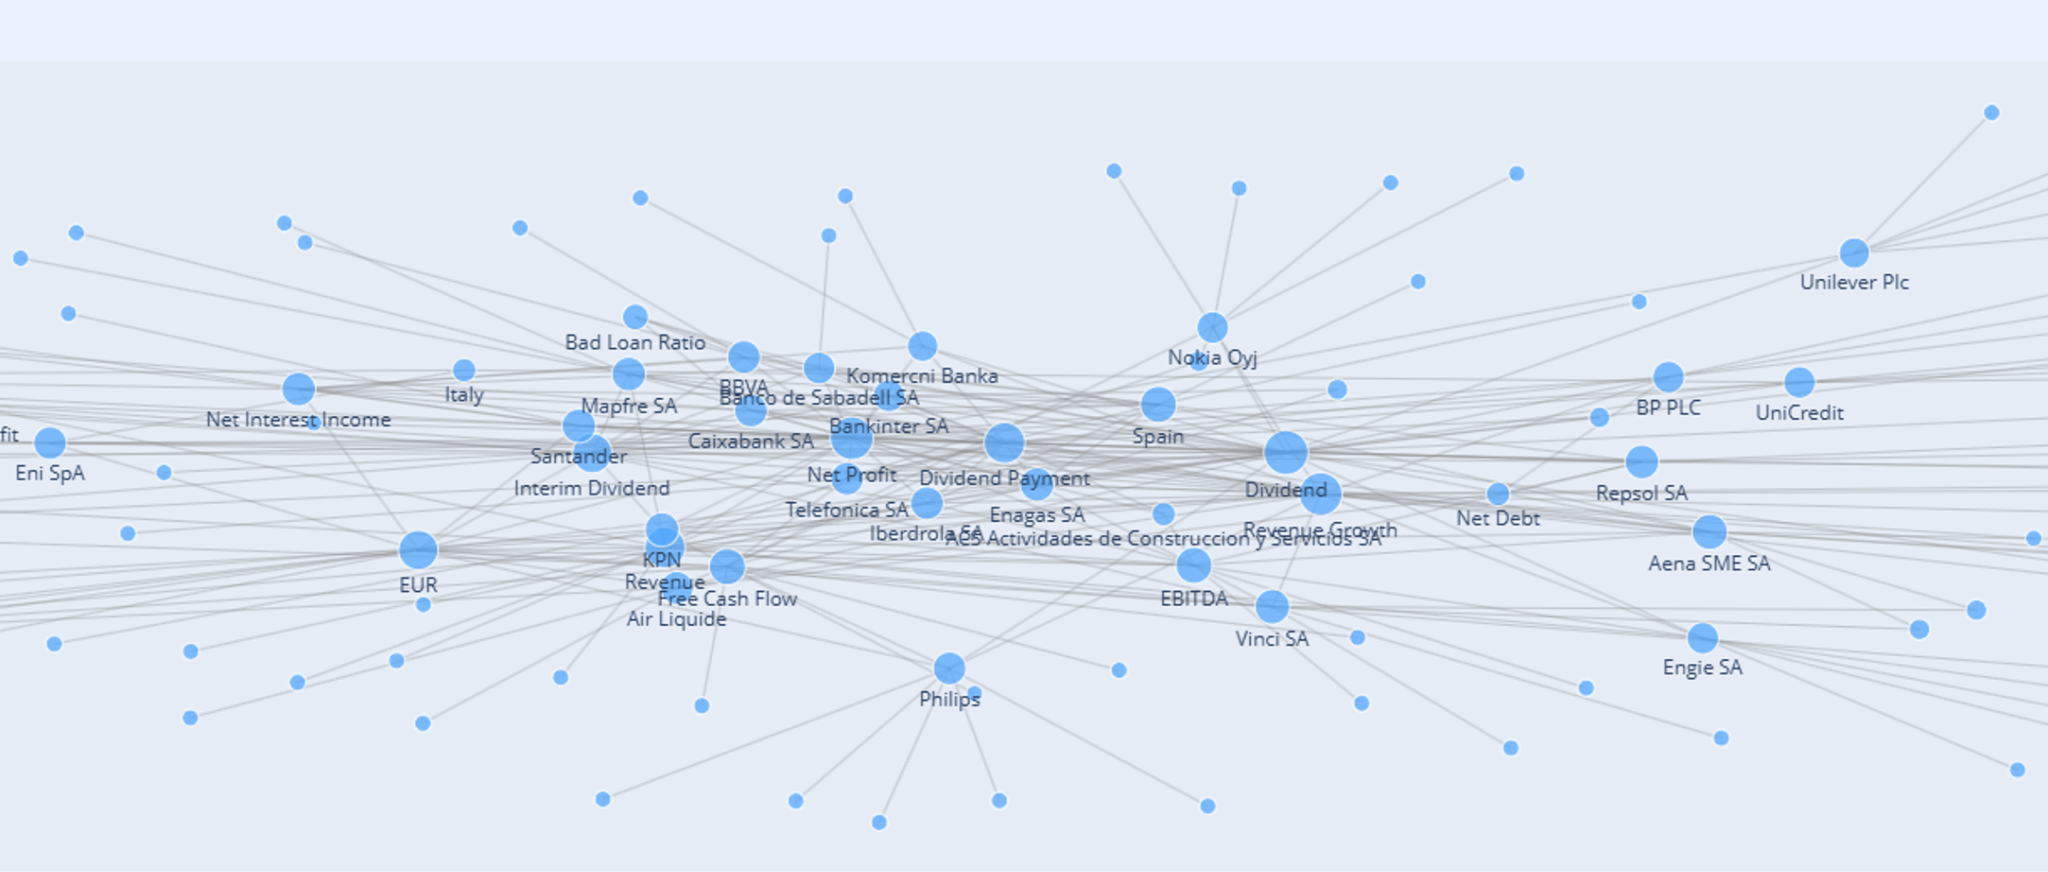
\includegraphics[width=0.95\textwidth]{figures/spring2025_kg.png}
\caption{Spring 2025: interactive Pyvis knowledge graph over European financial news --- companies, indicators and countries linked by extracted relations.}
\label{fig:spring2025kg}
\end{figure}

\subsection{Summer 2025 --- Metrics, Judge LLMs, regeneration}
\emph{Gunn Lee; Jarvis Gao; Xinnan Lu; Andrea Cuadros.}

\begin{itemize}
  \item Prompt engineering overhaul: 5-tuple \(\to\) \textbf{6-tuple} output adding a relationship-category type (GFMK / SSI / GMM); entity taxonomy 11 \(\to\) 14 types (adding DERIVATIVE, EQUITIES, MACRO\_INDICATOR) with refined definitions; few-shot examples 5 \(\to\) 8 with errors amended.
  \item \textbf{Handcrafted metrics} (unsupervised, lightweight): Coverage (MiniLM-L6-v2 embeddings, weighted cosine similarity), Semantic Uniqueness (similarity grouping; score = groups/triplets), Semantic Validity (ontology domain/range checks), Entropy Ratio (triplet vs.\ article information density; want \(<1\)).
  \item \textbf{Judge LLMs}: one independent judge per metric dimension, scoring 0--1 with a written explanation for interpretability.
  \item \textbf{Triplet regeneration pipeline} --- the origin of the project's three-LLM design: if any LLM metric falls below threshold, a third LLM (Gemini 2.5 Flash) regenerates the triplets from the original article plus the judge and handcrafted evaluations; handcrafted-below/LLM-above disagreements are flagged for human review.
  \item Dataset expansion: from \(\approx\)19k headline-only samples (\(\approx\)82 words each) to \(\approx\)11k full-article samples (\(\approx\)743 words) --- over 9\(\times\) more context per sample.
  \item Model comparison on identical inputs (Table~\ref{tab:summer2025eval}): Gemini 2.5 Flash beat Amazon Nova Pro on coverage (LLM coverage 0.893 vs.\ 0.735), comparable on uniqueness and validity.
\end{itemize}

\begin{table}[h]\centering\small
\begin{tabular}{lcc}
\toprule
Metric & Gemini 2.5 Flash & Amazon Nova Pro \\
\midrule
Handcrafted Coverage & 0.823 & 0.799 \\
LLM Coverage & 0.893 & 0.735 \\
Handcrafted Uniqueness & 0.584 & 0.768 \\
LLM Uniqueness & 0.941 & 0.974 \\
Handcrafted Semantic & 0.890 & 0.775 \\
LLM Semantic & 0.985 & 0.954 \\
Entropy Ratio & 0.735 & 0.679 \\
\bottomrule
\end{tabular}
\caption{Summer 2025 extraction-model evaluation, averaged over 10 samples per model (from the team's poster).}
\label{tab:summer2025eval}
\end{table}

\begin{figure}[h]\centering
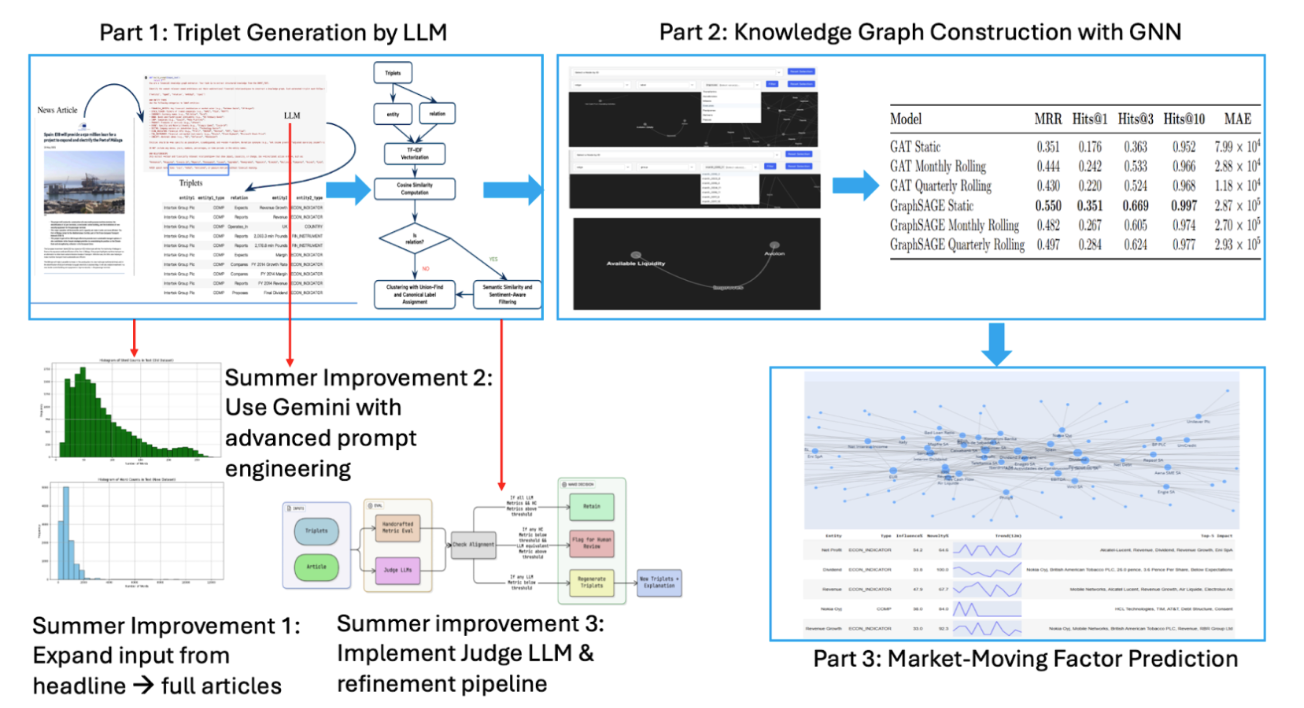
\includegraphics[width=0.9\textwidth]{figures/prior_work_overview.png}
\caption{Overview of the pre-Fall-2025 pipeline (from the Fall 2025 poster): triplet generation, knowledge-graph construction with GNNs, and market-moving factor prediction, with the three Summer 2025 improvements annotated.}
\label{fig:priorwork}
\end{figure}

\subsection{Fall 2025 --- FNSPID, local Qwen, unified pipeline}
\emph{Lee, G.; Gao, J.; Lu, X.; Cuadros, A.}

\begin{itemize}
  \item Ingested the FNSPID financial news dataset (Zihan1004 on Hugging Face).
  \item Restricted focus to semiconductor-related news (2020--2024).
  \item Extracted triplets using a locally-hosted Qwen 2.5 LLM via Ollama.
  \item Reverse-engineered the four Judge-LLM quality criteria into the initial extraction prompt itself --- shortcutting a slow generate-then-critique loop.
  \item Defined the four quality dimensions: Coverage, Uniqueness, Semantic Validity, Consistency.
  \item Built the first Graph Attention Network (GAT) for link prediction; trialled five loss functions (BPR, InfoNCE, Cross-Entropy, FindKG, Hybrid).
  \item Defined three graph-construction strategies keyed to Judge output: \emph{Original}, \emph{Fallback}, \emph{Strict}.
  \item Unified the pipeline end to end (Figure~\ref{fig:unifiedpipeline}): article-level handcrafted + Judge evaluation with regenerate-or-flag routing, then corpus-level frequency filtering, TF-IDF similarity clustering, union-find canonical mapping, relation-label consolidation and global dedupe.
  \item Switched to a locally hosted Qwen 2.5 32B via Ollama with a structured ``Mental Sandbox'' prompt --- rapid iteration, stable throughput, zero API cost.
  \item Key finding: \textbf{cleaner graphs beat larger ones}. The Strict graph, \(\approx\)58\% smaller than raw, reached the project's best MRR of 0.8018 (BPR loss, no edge features), improving Hits@1 by \(\approx\)10\%; ranking losses beat classification losses; topology carried more signal than relation semantics.
  \item Delivered interactive topology-aware visualisation of the monthly graphs (Figure~\ref{fig:fall2025graph}) plus global topology metrics tracked over time.
\end{itemize}

\begin{figure}[h]\centering
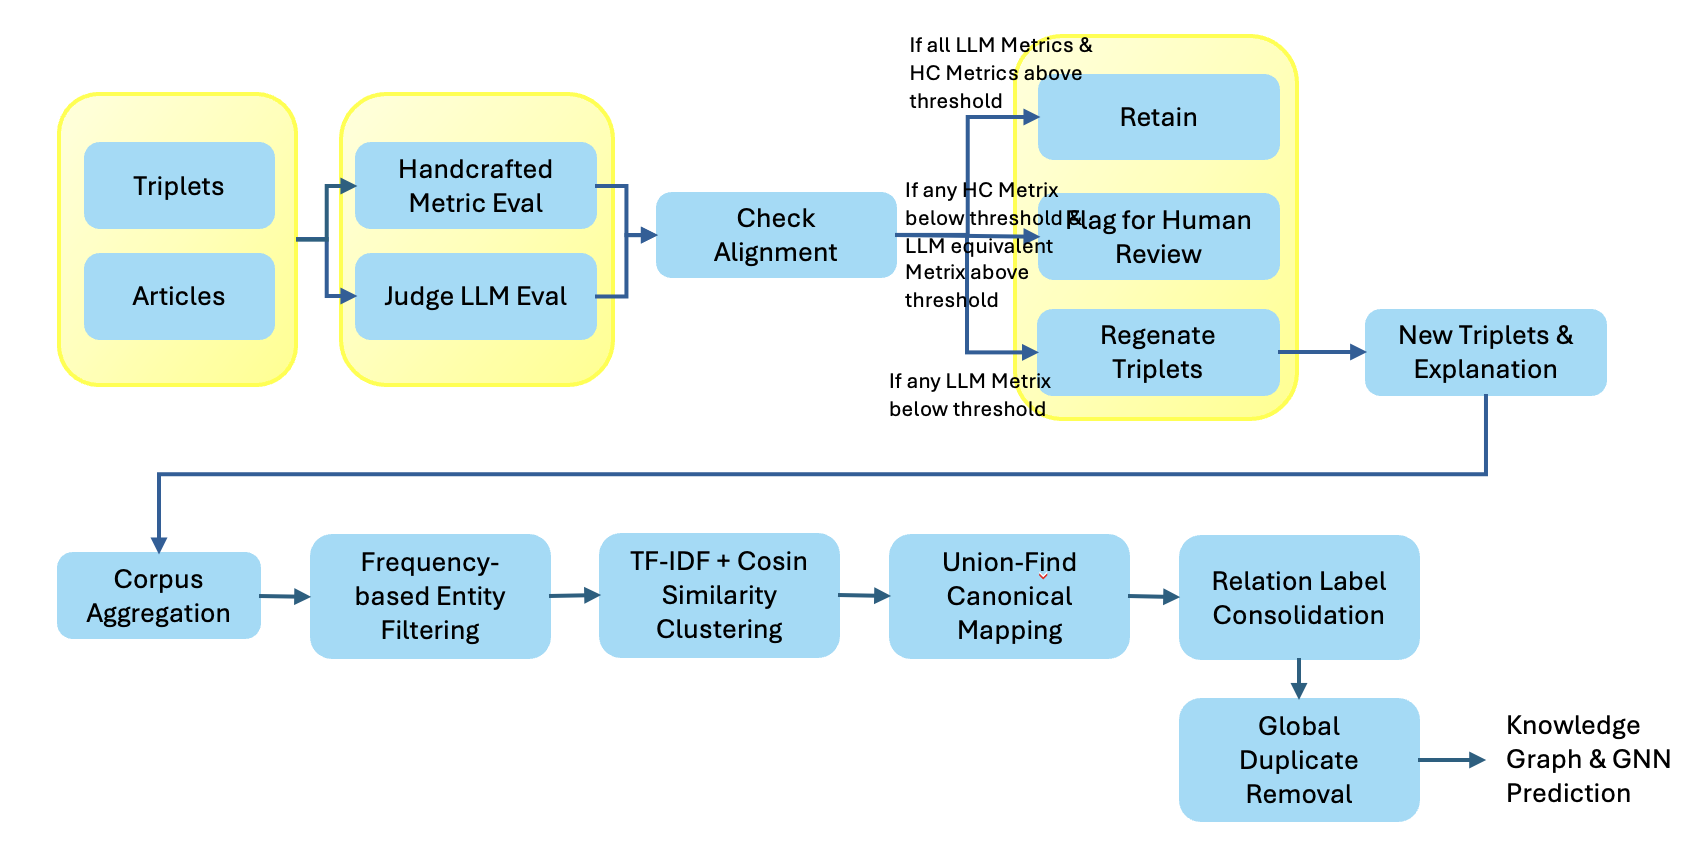
\includegraphics[width=0.95\textwidth]{figures/unified_pipeline.png}
\caption{Fall 2025 unified end-to-end pipeline: evaluation-gated retention / human review / regeneration at the article level, then corpus-level canonicalisation into the graph used for GNN prediction.}
\label{fig:unifiedpipeline}
\end{figure}

\begin{figure}[h]\centering
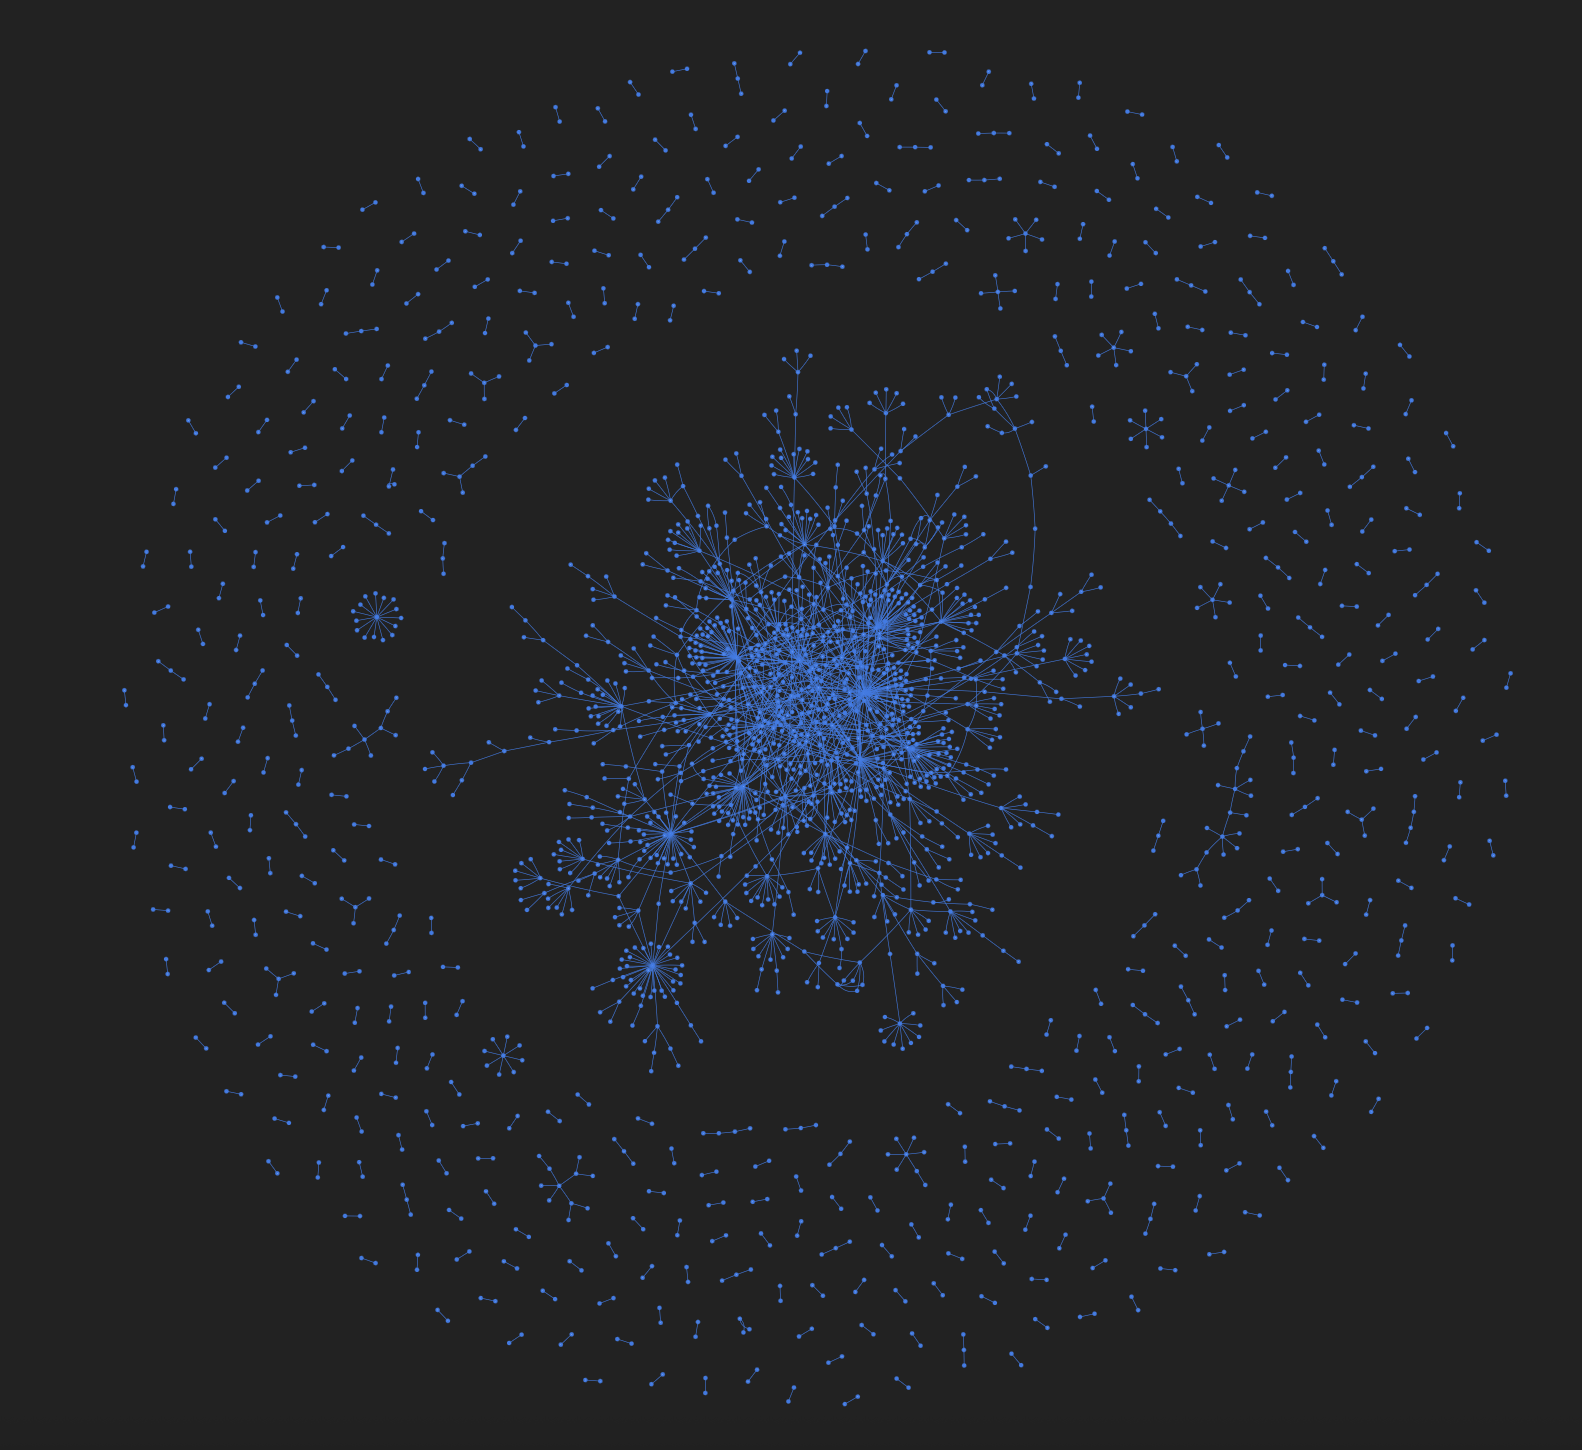
\includegraphics[width=0.8\textwidth]{figures/fall2025_full_graph.png}
\caption{Fall 2025: full knowledge graph over the FNSPID semiconductor corpus --- a dense connected core surrounded by small satellite stories.}
\label{fig:fall2025graph}
\end{figure}

\subsection{Spring 2026 --- Robustness and causality}
\emph{Xixi Chen; Xinyi Chen; Yi Yang.}

\begin{itemize}
  \item Systematically compared triplet extraction from \emph{full article text} versus \emph{article summary}. Full text won by \(\approx\) 0.08 MRR --- coverage dominates redundancy.
  \item Identified and fixed a temporal data-leakage bug in the rolling-window evaluation: the original code built its global entity index from the full dataset before splitting into train/test, so the model implicitly saw future entities through its embedding table.
  \item Ran a window-size ablation: 3-month training window beat 6-month and 12-month across every configuration --- recency dominates historical depth in a non-stationary market.
  \item Added \emph{causal feature augmentation}: encoded each entity's causal role (in-degree, out-degree, PageRank on a NOTEARS-learned DAG) as a 5-dimensional add-on to the 33-dimensional baseline features.
  \item Case-studied two market events: Covid-19 (gradual, 2019--2020) and the Russia--Ukraine war (sudden, 2021--2022).
    \begin{itemize}
      \item Covid-19: causal features cut the shock-period MRR drop by 96\%.
      \item Ukraine war: absolute performance higher; within-shock variance dramatically lower.
    \end{itemize}
  \item Consolidated the pipeline into a documented package with a Rolling Window subfolder for the corrected training code.
\end{itemize}

\subsection{Summer 2026 --- Comparison, UI, deployment}
\emph{Alexandra Paiz; Pierre Pujol (GitHub \href{https://github.com/SigmaWave}{SigmaWave}); Ruiwen Wang.}

\begin{itemize}
  \item Ran a controlled multi-model LLM benchmark on identical inputs: Claude Sonnet 5, GPT-5, Qwen 2.5 14B, Gemini 2.5 Flash. All extractions scored by the same Judge LLM (Qwen 2.5 14B via Ollama) on Coverage, Uniqueness, Semantic Validity, Consistency.
  \item Retrained the GAT on the 2019--2020 corpus with the Spring 2026 rolling-window fix; produced 230 checkpoints (10 model configurations \(\times\) 23 monthly validation periods).
  \item Built an interactive, publicly deployed web application (Next.js 16, Cytoscape.js, Tailwind CSS, shadcn/ui) at \url{https://eib-knowledge-graph.vercel.app}.
  \item Added a FinDKG-style ``Top KG Entities'' predictions leaderboard driven by real GAT embeddings, per month, exposing rank percentile, novelty z-score, 3-month trend sparkline, and top predicted-impacted financial entities.
  \item Deployed a self-updating news scraper framework (Google News RSS + regulator RSS feeds; GitHub Actions cron; per-corpus watchlists).
  \item Deployed static builds to Vercel with automatic redeploy on every push to \texttt{main}.
  \item Stood up a fully automated \textbf{live corpus} --- STOXX Europe 600, 30 curated tickers, refreshed daily by GitHub Actions with zero manual steps (Section~\ref{sec:stoxx}).
  \item Built a \textbf{news factor model} (five factors + PCA + KMeans archetype clustering) over the live corpus, exposed as a dedicated UI tab (Section~\ref{sec:factors}).
  \item Brought the extraction up to the three-LLM standard of the team pipeline: judge-and-refine pass plus cross-article entity canonicalisation (Section~\ref{sec:refinement}).
  \item Built the \textbf{VM-to-UI publishing pipeline} and used it to ship the full 2-year Qwen extraction (5{,}358 articles / 30{,}861 triplets) to the public UI (Section~\ref{sec:vmpipe}).
\end{itemize}

% =====================================================================
\section{Data}

\subsection{Source corpus}
\begin{itemize}
  \item \textbf{FNSPID} (Financial News and Stock Price Integration Dataset), Hugging Face \texttt{Zihan1004/FNSPID}.
  \item 15.7M financial news articles, 1999--2023, mapped to NASDAQ tickers.
  \item Full articles include title, body, ticker, timestamp, URL.
\end{itemize}

\subsection{Working subset for this project}
\begin{itemize}
  \item \textbf{Semiconductor slice} used throughout: \(\approx\) 2{,}300 articles across 2019--2020, chosen for its coverage of a full pre-shock / shock / post-shock cycle (Covid-19).
  \item Second slice used for the Spring 2026 causal study: \(\approx\) 2021--2022, spanning the Russia--Ukraine invasion.
\end{itemize}

\subsection{Extracted knowledge graph}
\begin{itemize}
  \item File: \texttt{summary\_triplets\_19\_20.csv} (Spring 2026 deliverable).
  \item \(\approx\) 11{,}800 triplets after quality filtering.
  \item \(\approx\) 8{,}000 unique entities across the 24 monthly snapshots.
  \item Entity types normalised to a closed vocabulary of 18 categories (company, stock ticker, sector, financial instrument, macro indicator, etc.).
\end{itemize}

% =====================================================================
\section{Pipeline overview}
\label{sec:pipeline}

Four sequential stages, unchanged in intent since Fall 2025, refined in every semester:

\begin{enumerate}
  \item \textbf{Triplet extraction.} LLM reads each news article, returns a list of \((\text{entity}_1, \text{type}_1, \text{relation}, \text{relation\ category}, \text{entity}_2, \text{type}_2)\) tuples.
  \item \textbf{Quality evaluation.} An independent Judge LLM scores each extraction on four dimensions and, if flagged, requests a revision.
  \item \textbf{Graph construction.} Triplets become edges of a directed graph; entities become nodes. One graph per calendar month.
  \item \textbf{Link prediction.} A Graph Attention Network is trained on trailing months and evaluated on the next month --- the ``predictable'' relationships become the model's output.
\end{enumerate}

% =====================================================================
\section{Stage 1 --- Triplet extraction}

\subsection{The triplet as unit of knowledge}
\begin{itemize}
  \item A triplet is one factual claim: ``\textit{Taiwan Semiconductor --- manufactures for --- AMD}''.
  \item Six-slot format: \((e_1, \text{type}_1, r, c, e_2, \text{type}_2)\) --- two entities, their types, the relationship verb, and the relationship's high-level category.
  \item Relationship categories collapse the hundreds of verbs into three families:
    \begin{itemize}
      \item \emph{SSI} --- Sector-Specific Insights (product launches, R\&D, deals).
      \item \emph{GMM} --- Global Market Movements (macro drivers, cross-market flows).
      \item \emph{GFMK} --- General Financial Market Knowledge (ownership, ticker mapping, structural facts).
    \end{itemize}
  \item Rationale: keep the vocabulary permissive at the verb level while giving downstream models a coarse handle on relationship meaning.
\end{itemize}

\subsection{Prompt engineering}
\begin{itemize}
  \item Prompt template lives in \texttt{components/tgp.txt} (triplet generation prompt).
  \item Instructs the model to: identify entities, classify each entity type against the ontology, propose the relationship verb, tag the category, avoid duplicates.
  \item The Fall 2025 team pre-loaded the four Judge criteria into this prompt --- so the extractor already tries to satisfy Coverage / Uniqueness / Validity / Consistency in a single pass.
\end{itemize}

\subsection{Models used across semesters}
\begin{itemize}
  \item \textbf{Fall 2025:} Qwen 2.5 (14B and 32B variants) locally via Ollama.
  \item \textbf{Spring 2026:} Same Qwen 2.5, focus was downstream not on the extractor.
  \item \textbf{Summer 2026:} Multi-model comparison --- Qwen 2.5 14B (baseline), Claude Sonnet 5, GPT-5, Gemini 2.5 Flash.
\end{itemize}

\subsection{Multi-LLM benchmark (Summer 2026)}
\begin{itemize}
  \item \textbf{Design.} Same 127-article slice of the corpus fed to each model; identical prompt; identical Judge LLM (Qwen 2.5 14B) scoring the outputs. Fully apples-to-apples.
  \item \textbf{Cost + speed.}
    \begin{itemize}
      \item Gemini 2.5 Flash: 129 articles, 1{,}213 triplets, \(\approx\)\$0.05, 18.7s / article average. 100\% well-formed output.
      \item Claude / GPT / Qwen: costs and speeds recorded in Pierre's benchmark deck.
    \end{itemize}
  \item \textbf{Robustness.} Signal.SIGALRM per-article timeout (60s) added to prevent silent hangs; incremental CSV checkpointing every 10 articles so an aborted run resumes cheaply.
  \item \textbf{Results} (see Section~\ref{sec:judge-results}) --- Gemini 2.5 Flash's Judge scores: Coverage 0.74, Uniqueness 0.83, Semantic Validity 0.84, Consistency 0.92 on 127 articles.
\end{itemize}

% =====================================================================
\section{Stage 2 --- Judge LLM quality evaluation}
\label{sec:judge}

\subsection{Motivation}
\begin{itemize}
  \item Raw LLM output is noisy: hallucinated entities, mis-typed entities, redundant triplets, contradictions.
  \item Feeding noise into the graph pollutes downstream training.
  \item Solution: a second LLM (the ``Judge'') re-reads each extraction and scores it.
  \item Judge is independent from the extractor to avoid confirmation bias.
\end{itemize}

\subsection{The four dimensions}

\textbf{Coverage} --- fraction of salient content in the source article captured by the triplet set.
\[
  \text{Coverage}(a) = \frac{|\{k \in \mathcal{K}_a \mid k\ \text{referenced by some}\ t_i \in \mathcal{T}_a\}|}{|\mathcal{K}_a|}
\]
where \(\mathcal{K}_a\) is the set of salient semantic units in article \(a\) and \(\mathcal{T}_a\) is the extracted triplet set.

\textbf{Uniqueness} --- penalises redundant triplets (measured via cosine similarity in embedding space):
\[
  \text{Uniqueness}(a) = 1 - \frac{2}{n(n-1)} \sum_{i<j} \mathbb{1}(\cos(\phi(t_i), \phi(t_j)) > \tau)
\]

\textbf{Semantic Validity} --- fraction of triplets that are semantically well-formed against the financial ontology:
\[
  \text{Validity}(a) = \frac{1}{n} \sum_{i=1}^n \mathbb{1}(t_i\ \text{is semantically valid})
\]

\textbf{Consistency} --- absence of pairwise contradictions:
\[
  \text{Consistency}(a) = 1 - \frac{|\{(t_i, t_j) \mid t_i \perp t_j\}|}{\binom{n}{2}}
\]

All four are in \([0, 1]\); higher is better.

\subsection{Three filtering strategies}
\begin{itemize}
  \item \textbf{Original.} Raw LLM output, no Judge intervention. Maximum recall, most noise.
  \item \textbf{Fallback.} Judge's revision applied where valid; falls back to the original if the revision is malformed. Balanced.
  \item \textbf{Strict.} Only triplets explicitly validated or corrected by the Judge kept. Maximum precision, smallest graph.
\end{itemize}

\subsection{Cross-model results (Summer 2026 benchmark)}
\label{sec:judge-results}

Gemini 2.5 Flash on the 127-article shared slice:

\begin{center}
\begin{tabular}{lrrrrr}
\toprule
\textbf{Dimension}   & \textbf{Mean} & \textbf{Median} & \textbf{Std} & \textbf{Min} & \textbf{Max} \\
\midrule
Coverage             & 0.74 & 0.70 & 0.07 & 0.60 & 0.90 \\
Uniqueness           & 0.83 & 0.80 & 0.10 & 0.60 & 1.00 \\
Semantic Validity    & 0.84 & 0.85 & 0.07 & 0.60 & 1.00 \\
Consistency          & 0.92 & 0.90 & 0.08 & 0.70 & 1.00 \\
\bottomrule
\end{tabular}
\end{center}

Full comparison table (Claude / GPT / Qwen / Gemini side-by-side) --- see Pierre's benchmark deck, EIB Report 4.

% =====================================================================
\section{Stage 3 --- Knowledge graph construction}

\subsection{From triplets to graph}
\begin{itemize}
  \item Nodes: distinct entities across all triplets in a given time window.
  \item Node attributes: entity type (company, sector, ticker, ...).
  \item Edges: directed, from \(e_1\) to \(e_2\). Attributes carry the verb and its category (SSI / GMM / GFMK).
  \item Edge weight: multiplicity --- how many articles support this exact relationship in the window.
\end{itemize}

\subsection{Temporal snapshots}
\begin{itemize}
  \item One graph per calendar month --- 24 snapshots for the 2019--2020 corpus.
  \item Each snapshot is a self-contained slice: nodes and edges only from articles dated that month.
  \item Design rationale: financial relationships are non-stationary --- what mattered in January 2020 is not what matters in April.
\end{itemize}

\subsection{Text vs.\ summary --- Spring 2026 finding}
\begin{itemize}
  \item Two graphs built from the same articles, one from the article body and one from an LLM-generated summary.
  \item \emph{Coverage} favoured full text substantially (0.778 vs.\ 0.687).
  \item \emph{Uniqueness} favoured the summary (0.918 vs.\ 0.874) --- summaries are naturally less redundant.
  \item Downstream GAT link prediction favoured the full-text graph consistently by \(\approx\) 0.08 MRR across all 10 model configurations.
  \item Conclusion: breadth beats precision for graph learning. Redundancy in the source is absorbed by the model; missing information cannot be.
\end{itemize}

\subsection{Static layout (Summer 2026)}
\begin{itemize}
  \item Node positions precomputed with \texttt{networkx.spring\_layout} at snapshot build time.
  \item Layout is deterministic --- the same month always renders in the same arrangement.
  \item Frontend consumes these positions directly (Cytoscape ``preset'' layout) so the graph appears at its final view instantly, no settling animation, no drift.
\end{itemize}

% =====================================================================
\section{Stage 4 --- Graph Attention Network}
\label{sec:gat}

\subsection{What the model is doing, in plain English}
\begin{itemize}
  \item Assign every entity a 256-dimensional vector (its ``meaning'').
  \item Update each entity's vector by attending to its neighbours in the graph, weighted by how relevant each neighbour looks.
  \item After training, similar vectors indicate the model thinks two entities relate to each other.
  \item ``Link prediction'' = ask the model: for entity \(A\), which unseen entities \(B\) does the model score highest? These are its predictions.
\end{itemize}

\subsection{Architecture}
\begin{center}
\begin{tabular}{ll}
\toprule
\textbf{Component} & \textbf{Configuration} \\
\midrule
Input linear       & 33 \(\to\) 256 (baseline) or 38 \(\to\) 256 (causal) \\
Node-type embed    & 256-dim, one per entity type \\
Node-id embed      & 256-dim, 0.5 dropout during training \\
LayerNorm          & After summing input + type + id \\
GATConv layer 1    & 256 \(\to\) 256, 4 heads concatenated, edge-dim 33 \\
GATConv layer 2    & 1024 \(\to\) 256, 1 head, mean aggregation \\
Edge features      & rel\_emb(16) + cat\_emb(16) + \(\log(1+w)\)(1) = 33-dim \\
\bottomrule
\end{tabular}
\end{center}

\subsection{Loss functions compared}
\begin{itemize}
  \item \textbf{BPR} (Bayesian Personalised Ranking) --- pairwise ranking: pull true edges above sampled negatives.
    \[ \mathcal{L}_{\text{BPR}} = -\frac{1}{N} \sum \ln \sigma(s(u, v^+) - s(u, v^-)) \]
  \item \textbf{InfoNCE} (contrastive) --- treat link prediction as a multi-class problem across \(K\) negatives.
    \[ \mathcal{L}_{\text{InfoNCE}} = -\log \frac{\exp(s(u, v^+)/\tau)}{\exp(s(u, v^+)/\tau) + \sum_i \exp(s(u, v_i^-)/\tau)} \]
  \item \textbf{CE} (Cross-Entropy) --- absolute link-existence probability.
    \[ \mathcal{L}_{\text{CE}} = -[y \log p + (1-y) \log(1-p)] \]
  \item \textbf{FindKG} --- the margin-based loss from the FinDKG paper.
  \item \textbf{Hybrid} --- CE + InfoNCE weighted combination.
\end{itemize}

\subsection{Rolling-window evaluation}
\begin{itemize}
  \item Train on months \([t - W, t]\), evaluate on month \(t + 1\), roll forward, repeat.
  \item For each true edge in the test month, sample 50 negatives; measure whether the model ranks the true one above the negatives.
  \item Metrics: MRR (Mean Reciprocal Rank), Hits@1, Hits@3, Hits@10.
  \item ``Seen'' vs.\ ``Unseen'' MRR reported separately --- edges between known-in-train entities vs.\ novel entities.
\end{itemize}

\subsection{Spring 2026 data-leakage fix}
\begin{itemize}
  \item Original bug: global entity index built from the entire dataset before splitting, so the embedding table implicitly contained future entities.
  \item Fix: build index only from the initial training window; update incrementally as the window rolls forward.
  \item Effect: honest evaluation --- previously optimistic MRRs came down; comparisons across window sizes and loss functions became apples-to-apples.
\end{itemize}

\subsection{Spring 2026 window-size ablation}

\begin{center}
\begin{tabular}{lrrrrr}
\toprule
\textbf{Config} & \textbf{Splits} & \textbf{MRR} & \textbf{H@1} & \textbf{H@3} & \textbf{H@10} \\
\midrule
3M train / 1M test  & 46 & \textbf{0.8126} & 0.7274 & 0.8740 & 0.9718 \\
6M train / 1M test  & 43 & 0.7934 & 0.6981 & 0.8561 & 0.9578 \\
6M train / 3M test  & 40 & 0.7891 & 0.6943 & 0.8512 & 0.9534 \\
12M train / 1M test & 37 & 0.7666 & 0.6727 & 0.8275 & 0.9483 \\
\bottomrule
\end{tabular}
\end{center}

\begin{itemize}
  \item Monotonic decline with longer training windows --- recency wins.
  \item Interpretation: financial knowledge graph structure is non-stationary; older windows drag in patterns from stale regimes.
  \item Practical implication: a 3-month rolling window costs less compute AND performs best.
\end{itemize}

\subsection{Spring 2026 causal augmentation}
\begin{itemize}
  \item Baseline node features (33-dim): 32-dim name hash + 1-dim log-degree.
  \item Causal add-on (5-dim): in-degree, out-degree, in-edge-weight-sum, out-edge-weight-sum, PageRank --- all computed on a DAG learned via NOTEARS.
  \item NOTEARS: continuous optimisation for learning directed acyclic graphs from observational data (Zheng et al., 2018).
  \item Applied to the top-200 most-mentioned entities to keep the co-occurrence matrix tractable.
  \item Hypothesis: causal roles are more stable than correlation patterns across market regimes.
\end{itemize}

\subsection{Causal augmentation results}
\begin{itemize}
  \item \textbf{Covid-19 (2019--2020).} Baseline MRR fell 0.0763 from pre-shock to shock. Causal model fell only 0.0031 --- a 96\% reduction in shock drop.
  \item \textbf{Ukraine war (2021--2022).} Causal model absolute performance higher across all phases (pre-MRR 0.7290 vs.\ 0.6853). Within-shock standard deviation drops by \(\approx\) 6\(\times\) (MRR \(\sigma\) 0.0026 vs.\ 0.0152).
  \item \textbf{Trade-off.} Causal features add \emph{noise} during stable periods (small MRR sacrifice) in exchange for shock resilience.
  \item \textbf{Interpretation.} Causal features help most when the disruption is preceded by detectable shifts in news coverage (Covid); help less for sudden exogenous shocks with no prior signal (war).
\end{itemize}

\subsection{Summer 2026 rerun}
\begin{itemize}
  \item Retrained the full 10-configuration leaderboard on the 2019--2020 corpus using the Spring 2026 rolling-window fix.
  \item Ran on CPU (Apple MPS backend crashed with a known Metal assertion on this graph size).
  \item Wall time: \(\approx\) 19 minutes for the full sweep (10 configs \(\times\) 23 validation months).
  \item Winner: \textbf{CE (No Edge Feats), MRR 0.7746}.
  \item Full leaderboard:
\end{itemize}

\begin{center}
\begin{tabular}{rlrrrr}
\toprule
\textbf{Rank} & \textbf{Model} & \textbf{MRR} & \textbf{H@1} & \textbf{H@3} & \textbf{H@10} \\
\midrule
1  & CE (No Edge Feats)       & \textbf{0.7746} & 0.6891 & 0.8235 & 0.9463 \\
2  & BPR (No Edge Feats)      & 0.7465 & 0.6596 & 0.7938 & 0.9182 \\
3  & InfoNCE (Rel+Cat+NormW)  & 0.7455 & 0.6662 & 0.7869 & 0.8988 \\
4  & InfoNCE (No Edge Feats)  & 0.7392 & 0.6595 & 0.7768 & 0.8969 \\
5  & Hybrid (No Edge Feats)   & 0.7334 & 0.6441 & 0.7828 & 0.9092 \\
6  & CE (Rel+Cat+NormW)       & 0.7257 & 0.6357 & 0.7738 & 0.9058 \\
7  & BPR (Rel+Cat+NormW)      & 0.7194 & 0.6302 & 0.7637 & 0.9006 \\
8  & FindKG (No Edge Feats)   & 0.7167 & 0.6184 & 0.7716 & 0.9135 \\
9  & FindKG (Rel+Cat+NormW)   & 0.7049 & 0.6054 & 0.7622 & 0.9077 \\
10 & Hybrid (Rel+Cat+NormW)   & 0.7036 & 0.6083 & 0.7575 & 0.8907 \\
\bottomrule
\end{tabular}
\end{center}

\begin{itemize}
  \item Interpretation of MRR 0.77: on average the true target entity is ranked \(\approx\) 1.3 out of 51 candidates. Random baseline would be \(\approx\) 0.05.
  \item Edge features (relationship type + category) do not consistently help --- graph topology alone carries most of the signal.
  \item Weights saved per (loss function, edge-feature setting, month) --- 230 checkpoint files.
\end{itemize}

% =====================================================================
\section{Predictions layer (Summer 2026)}
\label{sec:predictions}

\subsection{Design}
\begin{itemize}
  \item Modelled on the FinDKG paper's ``Top KG Entities'' leaderboard (Ago et al., 2024).
  \item One row per top entity, per month, per column of information --- see Section~\ref{sec:predictions-cols}.
  \item Backed by the actual winning GAT weights (CE No-Edge-Feats), not synthetic.
  \item Exposed in the UI as a full-height tab alongside the graph view.
\end{itemize}

\subsection{Columns}
\label{sec:predictions-cols}

\begin{itemize}
  \item \textbf{Top KG Entity.} The most influential entity in the month's graph, per the GAT.
  \item \textbf{Entity Type.} Company / sector / ticker / instrument / indicator (colour-coded chip).
  \item \textbf{Rank Percentile.} 0--100. Position of this entity when all entities are sorted by mean outgoing GAT prediction score.
  \item \textbf{Novelty (z-score).} Standardised measure of how spiking this entity's activity is versus its own historical baseline. Positive = spiking; near-zero = business as usual; negative = quieting.
    \[ \text{novelty}(e) = \frac{r(e) - \mu_r}{\sigma_r},\quad r(e) = \text{edges}_{\text{recent 3mo}}(e) - \overline{\text{edges}_{\text{prior}}}(e) \]
  \item \textbf{Recent 3-mo Trend.} Sparkline of edge counts in months \([P-2, P-1, P]\).
  \item \textbf{Predicted Most Impacted Financial Entities.} Top 5 targets by GAT score, filtered to financial entity types.
\end{itemize}

\subsection{Pipeline}
\begin{itemize}
  \item For each validation month with a GAT checkpoint:
    \begin{enumerate}
      \item Rebuild the month's graph.
      \item Load the CE No-Edge-Feats weights for that month.
      \item Run inference: produce 256-dim embedding per node.
      \item All-pairs dot product \(\to\) score matrix.
      \item Rank entities by mean outgoing score; compute percentile, novelty, trend, impacted list.
    \end{enumerate}
  \item All 23 monthly leaderboards baked into a single 446 KB static JSON at build time.
  \item UI fetches once, caches in-memory, and re-renders per selected month with zero backend calls.
\end{itemize}

\subsection{Reality check on the data}
\begin{itemize}
  \item Nothing is LLM-generated for these leaderboards. Trend and novelty are recomputed directly from the source CSV; ranking and impacted-entity lists come from real PyTorch weight files (\(\approx\) 10 MB each).
  \item Verified: for Texas Instruments in March 2020, novelty +3.05 and trend [13, 12, 2] both reproduce exactly from the source data.
  \item Failure modes visible in the output: extraction noise (stray numeric entities), duplicate entities (e.g.\ ``TXN'' and ``Texas Instruments Inc'' treated as separate nodes). These are upstream extraction issues, not prediction-layer issues.
\end{itemize}

% =====================================================================
\section{User interface (Summer 2026)}
\label{sec:ui}

\subsection{Design goals}
\begin{itemize}
  \item Non-technical analysts should be able to browse the knowledge graph without training.
  \item Every claim in the UI must be traceable to a source (article or model output), not a black-box statement.
  \item Deployable as a static site so it runs from Vercel's CDN with no backend infrastructure to maintain.
  \item Aesthetically restrained --- optimised for reading in a briefing setting.
\end{itemize}

\subsection{Architecture}
\begin{itemize}
  \item \textbf{Frontend:} Next.js 16 (App Router) + TypeScript, Cytoscape.js for graph rendering, Tailwind CSS for styling, shadcn/ui for primitives, next-themes for light/dark.
  \item \textbf{Data layer:} static JSON files under \texttt{/data/} (index, per-month snapshots, per-month article corpora, GAT predictions).
  \item \textbf{Optional backend:} FastAPI + Python for local pipeline re-runs and chat; not required in production.
  \item \textbf{Hosting:} Vercel personal account, auto-deploy on push to \texttt{main}. Domain: \texttt{eib-knowledge-graph.vercel.app}.
\end{itemize}

\subsection{Features}
\begin{itemize}
  \item \textbf{Interactive knowledge graph.} Pan, zoom, hover for edge tooltips, click a node to focus its neighbourhood (dim the rest).
  \item \textbf{Filter rail.} Toggle entity types on/off; toggle relationship categories; minimum-connections slider (proportional to the current view's max degree).
  \item \textbf{Time slider.} Dual-thumb date range. Preset chips: 1M / 3M / 6M / 12M / All. Defaults to trailing 6 months. Timeline slider drives BOTH the graph tab and the predictions tab.
  \item \textbf{Safari-style tabs.} Knowledge graph / Predictions. Only one visible at a time; state preserved on switch (with a Cytoscape lifecycle fix for the fit-viewport race condition).
  \item \textbf{Predictions view.} FinDKG-style table as described in Section~\ref{sec:predictions}.
  \item \textbf{Entity search (\(\mathcal{C}\)K).} Command-palette-style entity picker across the current snapshot.
  \item \textbf{Article search.} Keyword search across the source news corpus (per-month JSON bundles fetched in parallel, scored client-side).
  \item \textbf{Chat panel.} Optional LLM chat over the corpus (backend-only; user supplies their own API key).
  \item \textbf{Physics settings.} Optional d3-force live simulation for the graph, behind a gear icon. Off by default --- static precomputed positions are the default view.
  \item \textbf{Theme.} Light mode by default; dark mode toggle in the header.
\end{itemize}

\subsection{Recent UI iterations (Summer 2026, chronological)}
\begin{itemize}
  \item Replaced polarity edge colouring with 8-family causal-type colouring (Okabe--Ito colourblind-safe palette).
  \item Fixed graph layout to precomputed \texttt{spring\_layout} positions --- no more settle-from-chaos on page load.
  \item Added dual-thumb date range selector with client-side snapshot merging.
  \item Added Safari-style tab strip; predictions moved from a bottom drawer into a full tab.
  \item Removed purple / neon accents; migrated to neutral palette.
  \item Fixed Cytoscape crash on tab switch: cancelled pending \texttt{requestAnimationFrame} on unmount.
\end{itemize}

\subsection{Late-Summer 2026 overhaul}
\begin{itemize}
  \item \textbf{Multi-source architecture.} A source catalogue drives a data-source dropdown; each source declares which tabs it supports (FNSPID: graph + predictions; STOXX: graph + factor analysis; VM run: graph). Unsupported tabs are hidden, not greyed. Per-source data lives under \texttt{/data/sources/\(\langle\)id\(\rangle\)/}.
  \item \textbf{Timeline redesign.} Months are equal cells of the track (a 1-month selection is a full cell, not a point). The selected range is a visible window block: drag the middle to slide through time (glides with the pointer, snaps to month boundaries), drag the edges to resize, click the track to jump; preset chips 1M/3M/6M/12M/All; default trailing quarter. On the Predictions tab the same track shows the training months (amber) vs.\ the predicted month (emerald) of the rolling-window GAT.
  \item \textbf{Obsidian-style graph layout.} A real d3-force simulation runs to convergence before render: many-body repulsion, degree-scaled link springs, a collision force guaranteeing zero node overlap, and centring gravity. Deterministic (seeded), so a given view always lays out identically.
  \item \textbf{Readability at scale.} Node and label sizes are zoom-compensated to constant pixel size across corpora; node size normalised to each snapshot's own degree ceiling; permanent labels allocated by a collision-avoiding budget (all names in moderate or multi-cluster views, top-40\% in dense single-blob views, every cluster's top entity always named); auto density threshold targets the \(\approx\)300 most-connected nodes rather than a fixed percentage of the maximum degree.
  \item \textbf{Industry filter (STOXX).} A sector section above the entity-type checkboxes. Sectors are inferred per news cluster from the watchlist company it concerns; default view opens on Pharma with the other five sectors one click away.
  \item \textbf{Factor analysis tab.} As described in Section~\ref{sec:factors}.
  \item \textbf{Dead-control hygiene.} Controls that do not affect a given tab are hidden there (Factor analysis shows neither the filter rail nor the timeline).
  \item \textbf{Report tab.} This report, viewable in-app as an embedded PDF.
\end{itemize}

\subsection{Data flow diagram}
\begin{center}
\begin{tabular}{lcl}
News articles (FNSPID)      & \(\to\) & Triplet extraction (LLM) \\
Triplets                    & \(\to\) & Judge LLM quality scoring \\
Scored triplets             & \(\to\) & Monthly graph snapshots \\
Snapshots                   & \(\to\) & GAT rolling-window training \\
GAT weights                 & \(\to\) & Per-month predictions leaderboard \\
All artefacts (JSON)        & \(\to\) & Static Vercel deployment \\
                            &         & \(\downarrow\) \\
                            &         & Browser fetches JSON, renders UI \\
\end{tabular}
\end{center}

% =====================================================================
\section{Live corpus --- STOXX Europe 600 pipeline (Summer 2026)}
\label{sec:stoxx}

\subsection{Motivation}
\begin{itemize}
  \item Everything upstream operated on a fixed historical corpus. Question: can the whole chain --- fetch, extract, build graph, deploy --- run \emph{live}, unattended?
  \item Chosen universe: STOXX Europe 600 subset. European coverage is directly sponsor-relevant (EIB).
  \item Scope deliberately small: 30 curated tickers across six sectors (pharma, tech, banks, industrials \& autos, energy, consumer \& luxury) so a full daily run fits comfortably in a GitHub Actions job.
\end{itemize}

\subsection{Daily pipeline (fully automated)}
\begin{itemize}
  \item GitHub Actions cron, 07:30 UTC daily. No human in the loop; verified self-healing over multiple days (auto-commit with pull-rebase retry when other pushes land mid-run).
  \item Steps: fetch Google News RSS per ticker \(\to\) drop stale republished articles (\(>\)120 days old --- these previously spawned junk one-article months as far back as 2019) \(\to\) dedupe against a URL ledger \(\to\) Gemini 2.5 Flash extraction \(\to\) refinement passes (Section~\ref{sec:refinement}) \(\to\) merge into monthly snapshots \(\to\) recompute factor bundle \(\to\) commit. The commit triggers the Vercel redeploy.
  \item \textbf{Enriched extraction schema.} Each triplet carries three extra fields beyond subject/relation/object: sentiment \([-1,1]\), materiality (US-dollar magnitude mentioned with the fact), and an event-type tag. These feed the factor model.
  \item \textbf{Raw triplet persistence.} Every article's exact triplet list is stored per month before aggregation (\texttt{triplets/YYYY-MM.json}) --- article-level provenance, exact factor recomputation, and a future retraining dataset.
  \item Index hygiene: months whose snapshot holds fewer than 3 edges are excluded from the timeline (stray misdated articles cannot pollute the axis).
  \item Cost: on the order of cents per day (Gemini 2.5 Flash over \(\approx\)90 title-length articles). Runs until the API key is retired; the site then simply stops updating and keeps serving the last state.
  \item Known limitation: Google News RSS supplies titles only (\(\approx\)60 characters of signal per article) and no deep history --- the corpus accumulates forward from activation.
\end{itemize}

% =====================================================================
\section{Extraction refinement --- three-LLM parity (Summer 2026)}
\label{sec:refinement}

\begin{itemize}
  \item The team pipeline (Fall 2025 onward) is a \textbf{three-LLM design}: (1) a triplet-extraction LLM; (2) a Judge LLM scoring each article's triplets on coverage, uniqueness and semantic validity; (3) a \emph{flagged-triplet refinement} LLM that receives the article, the bad triplets and the judge's verdict, and regenerates better ones.
  \item The live pipeline initially ran stage 1 only (plus regex filters) --- the source of duplicate entities (``ASML'' / ``ASML Holding'' / ``ASML Holding N.V.'') and nonsense nodes (bare numbers, generic phrases).
  \item Now added, adapted to the title-only corpus and collapsed for cost:
  \begin{itemize}
    \item \textbf{Judge-and-refine pass} (one Gemini call per article). Drops entities that are meaningless as graph nodes, merges restated facts, normalises names within the article.
    \item \textbf{Cross-article entity canonicalisation} (one call per run). Maps name variants onto one canonical name each, preferring names already in the corpus so new edges merge into existing nodes instead of duplicating them. Tickers are never merged into companies.
  \end{itemize}
  \item Both passes \emph{fail open}: an API or parse failure keeps the first-pass triplets, so a flaky call degrades quality for a day rather than losing data.
\end{itemize}

% =====================================================================
\section{News factor model (Summer 2026)}
\label{sec:factors}

\subsection{Idea}
\begin{itemize}
  \item First-principles question: beyond drawing a graph, what is the \emph{analytical} utility of daily triplets? Answer: treat news coverage itself as a measurable signal --- a Fama--French-style factor decomposition of the news, per entity.
  \item Every company/topic in the corpus is scored on five factors, i.e.\ five plain questions about its recent coverage:
  \begin{itemize}
    \item \textbf{Attention} --- how much is it written about?
    \item \textbf{Sentiment} --- is the tone positive or negative?
    \item \textbf{Consensus} --- do sources agree, or is the story contested?
    \item \textbf{Novelty} --- is it generating its own storylines or only appearing in others'?
    \item \textbf{Materiality} --- how much money do its stories involve (deal sizes, fines, revenue figures)?
  \end{itemize}
\end{itemize}

\subsection{Method}
\begin{itemize}
  \item Factors roll up from the last two months of stored snapshots (a rolling corpus), not just the day's new articles --- the daily delta after ledger warm-up is a handful of articles and produced empty bundles until this fix.
  \item Scores standardised to z-scores; \textbf{KMeans} (\(k=5\)) clusters entities in the full five-factor space --- no sector labels or company information supplied. Clusters read as automatically discovered \emph{news archetypes}.
  \item Observed clusters are economically sensible: e.g.\ Novo Nordisk / Shell / Volkswagen form the high-attention--low-consensus group (heavily covered, contested stories); an energy-heavy cluster (BP, Eni) carries the high-materiality--positive-sentiment signature.
  \item \textbf{PCA} projects the five scores to two axes for display only (\(\approx\)76\% of variance in three components); clustering happens in the full space.
  \item UI: dedicated ``Factor analysis'' tab --- labelled scatter (collision-avoided names, zoom/pan with constant-size labels so overlaps separate on zoom), archetype cluster cards with plain-language signatures, and a collapsible analyst explainer covering what the tab is for, the factors, the clusters and the map, in non-engineer language.
\end{itemize}

% =====================================================================
\section{VM-to-UI publishing pipeline (Summer 2026)}
\label{sec:vmpipe}

\begin{itemize}
  \item The team's production extraction runs on a Google Cloud VM (\texttt{eib-central1a}; Ollama + Qwen 2.5 14B; tmux-detached runs over the full FNSPID corpus). Outputs accumulated on the VM with no path to the UI.
  \item Built \texttt{scripts/publish\_vm\_output.py}: converts the pipeline's output CSVs (article rows with 6-tuple triplets) into the site's data format --- monthly snapshots with layout positions, article records, raw triplet provenance --- and pushes; the push triggers the Vercel redeploy. Safe re-publish semantics (\texttt{--replace}), dry-run mode, tolerant CSV parsing for large files.
  \item \textbf{First production use.} The full 2019--2021 extraction (Qwen 2.5 14B, pushed to the team pipeline repository on 16 Aug) was published as a third UI source: \emph{FNSPID --- qwen2.5 VM run (2019--2021)}. 5{,}358 articles, 30{,}861 triplets, all 25 months browsable.
  \item Kept separate from the original FNSPID source so the GAT predictions remain consistent with the extraction they were trained on.
  \item Documented one-time VM setup (write-scoped deploy key + one cron line) in \texttt{docs/VM\_PUBLISHING.md}; alternatively a repository-side mirror workflow can poll the public pipeline repo for new outputs, requiring nothing from the VM at all.
\end{itemize}

% =====================================================================
\section{Deployment and infrastructure}

\begin{itemize}
  \item \textbf{Repository.} \url{https://github.com/ap4509-columbia/eib-knowledge-graph} (team collaborators: SigmaWave, Ruiwen04).
  \item \textbf{Vercel project.} \texttt{eib-knowledge-graph}. Auto-deploy on push to \texttt{main}. Aliased domains: \texttt{eib-knowledge-graph.vercel.app} + Git-branch preview URLs.
  \item \textbf{Static-only production build.} No backend at runtime. All data ships as JSON files served from the CDN.
  \item \textbf{Self-updating scraper} (live in production for the STOXX corpus --- Section~\ref{sec:stoxx}).
    \begin{itemize}
      \item Sources: Google News RSS (per-corpus watchlists), ECB / ESMA / BoE regulator RSS feeds.
      \item Per-corpus watchlists: US semiconductors, EU utilities, EU banks, EU regulators, STOXX Europe 600 (30-ticker curated subset in production).
      \item Deduplication ledger prevents re-processing.
      \item Runs daily as a GitHub Actions cron and auto-commits new snapshots; each commit triggers the Vercel redeploy.
    \end{itemize}
  \item \textbf{Local backend} (optional). FastAPI + uvicorn on port 8000 for pipeline re-runs and chat during development.
\end{itemize}

% =====================================================================
\section{Team contributions summary}

\begin{longtable}{p{0.22\textwidth} p{0.28\textwidth} p{0.44\textwidth}}
\toprule
\textbf{Team / semester} & \textbf{Members} & \textbf{Key contributions} \\
\midrule
Fall 2025 & Lee, Gao, Lu, Cuadros & \begin{itemize}
    \item Baseline end-to-end pipeline
    \item Triplet extraction prompt + ontology
    \item Judge LLM design (4 dimensions, 3 strategies)
    \item First GAT for link prediction
    \item Basic HTML visualisation
  \end{itemize} \\
\midrule
Spring 2026 & Xixi Chen, Xinyi Chen, Yi Yang & \begin{itemize}
    \item Full-text vs.\ summary extraction study
    \item Rolling-window data-leakage fix
    \item 3M / 6M / 12M window ablation
    \item Causal feature augmentation via NOTEARS
    \item Covid-19 + Ukraine war event studies
  \end{itemize} \\
\midrule
Summer 2026 & Alexandra Paiz, Pierre Pujol, Ruiwen Wang & \begin{itemize}
    \item Multi-model LLM benchmark (Claude / GPT / Qwen / Gemini)
    \item Interactive web application (Next.js + Cytoscape)
    \item FinDKG-style predictions leaderboard
    \item GAT retraining with fixed rolling window (MRR 0.7746)
    \item Self-updating scraper framework
    \item Vercel deployment
  \end{itemize} \\
\bottomrule
\end{longtable}

% =====================================================================
\section{Deliverables}

\subsection{Fall 2025}
\begin{itemize}
  \item \texttt{summary\_triplets\_metrics\_22.csv} --- earlier scored triplet dump.
  \item Original pipeline modules under \texttt{components/}.
  \item Static per-month HTML visualisations.
\end{itemize}

\subsection{Spring 2026}
\begin{itemize}
  \item Written report: \emph{LLM and Graphs for Financial Texts} (EIB1\_Report.pdf, 16 pages).
  \item Poster.
  \item \texttt{summary\_triplets\_19\_20.csv} --- the 2-year triplet corpus this project has used ever since.
  \item Corrected rolling-window code (\texttt{Rolling Window/} folder).
  \item NOTEARS causal feature pipeline (\texttt{causal\_files/} folder).
\end{itemize}

\subsection{Summer 2026}
\begin{itemize}
  \item Deployed web application: \url{https://eib-knowledge-graph.vercel.app}.
  \item Source repository (private).
  \item Multi-LLM benchmark: 4-model comparison + Judge LLM stats.
  \item Retrained GAT: 230 checkpoints + leaderboard CSV.
  \item Predictions JSON: 23 monthly leaderboards, 446 KB.
  \item Self-updating scraper framework + per-corpus watchlists.
  \item This report.
\end{itemize}

% =====================================================================
\section{Future work}

\subsection{Corpus extension}
\begin{itemize}
  \item Currently 2 years of triplets (2019--2020). The underlying FNSPID dataset extends 1999--2023 with \(\approx\) 15M articles.
  \item Extending to 5 years: \(\approx\)\$30 in LLM extraction cost, 2--3 days of processing.
  \item Extending to full 15 years: \(\approx\)\$200.
  \item Blocker: team budget decision, pending.
\end{itemize}

\subsection{Cross-industry expansion}
\begin{itemize}
  \item Current focus: semiconductors.
  \item Watchlists already defined for EU utilities, EU banks, EU regulators, STOXX Europe 600.
  \item Enables sponsor-relevant coverage (European infrastructure, regulation, banking).
\end{itemize}

\subsection{Sponsor-facing improvements}
\begin{itemize}
  \item Entity aliasing (dedupe ``TXN'' and ``Texas Instruments Inc'') --- \emph{shipped for the live corpus} via the canonicalisation pass (Section~\ref{sec:refinement}); extending it to the historical FNSPID sources is a one-off batch job over the now-persisted raw triplets.
  \item Currency numeral cleanup (bare numbers like ``1840'' as CURRENCY entities) --- \emph{shipped for the live corpus} via hard filters + the refine pass; pending for historical sources.
  \item Promote unmodelled entity types (PERSON, COUNTRY, LOCATION, INSTITUTION) to first-class schema types.
  \item Sentiment scores from Marketaux or equivalent as a second signal alongside triplets.
\end{itemize}

\subsection{Model integration}
\begin{itemize}
  \item Per-edge GAT confidence exposed as an ``uncertainty'' colour mode on the graph.
  \item Similar-entity retrieval from the node embeddings in the detail panel.
  \item Predicted \emph{new} edges (not just ranking known ones) drawn on the graph with a distinct style.
\end{itemize}

\subsection{Additional event studies}
\begin{itemize}
  \item Interest-rate cycles.
  \item European energy price spike (2022--2023).
  \item Banking-sector stress episodes.
\end{itemize}

% =====================================================================
\appendix

\section{Metric definitions --- quick reference}

\begin{itemize}
  \item \textbf{MRR} (Mean Reciprocal Rank). \(\text{MRR} = \frac{1}{|Q|} \sum_{q \in Q} \frac{1}{\text{rank}_q}\). Where \(\text{rank}_q\) is the position of the true target for query \(q\).
  \item \textbf{Hits@k}. Fraction of queries where the true target is in the top \(k\).
  \item \textbf{Coverage}. Fraction of salient article content captured by the extracted triplets.
  \item \textbf{Uniqueness}. \(1 -\) redundancy rate among the triplets (cosine similarity in embedding space).
  \item \textbf{Semantic Validity}. Fraction of triplets that fit the financial ontology.
  \item \textbf{Consistency}. Absence of pairwise contradictions.
  \item \textbf{Novelty z-score}. Standardised measure of an entity's activity spike vs.\ its own history.
  \item \textbf{Rank Percentile}. Position of an entity when ranked by mean outgoing GAT prediction score, expressed as a percentile.
\end{itemize}

\section{Software stack --- full list}

\begin{itemize}
  \item \textbf{Extraction:} Python, Ollama (Qwen 2.5 14B / 32B), Google Gemini API (google-genai), Anthropic API, OpenAI API.
  \item \textbf{Modelling:} PyTorch, PyTorch Geometric, NetworkX, SciPy, scikit-learn (PCA, KMeans), SentenceTransformers.
  \item \textbf{Backend:} FastAPI, uvicorn, pandas.
  \item \textbf{Frontend:} Next.js 16, TypeScript, Cytoscape.js, cytoscape-d3-force, Tailwind CSS, shadcn/ui, next-themes, lucide-react.
  \item \textbf{Infrastructure:} GitHub, GitHub Actions (cron), Vercel (deployment, CDN).
\end{itemize}

% =====================================================================
\begin{thebibliography}{9}
\bibitem{findkg}
Ago, T.\ et al.\ (2024). \emph{FinDKG: Dynamic Knowledge Graphs with Large Language Models for Detecting Global Trends in Financial Markets.} \url{https://arxiv.org/abs/2407.10909}

\bibitem{notears}
Zheng, X., Aragam, B., Ravikumar, P., \& Xing, E.\ P.\ (2018). \emph{DAGs with NO TEARS: Continuous optimization for structure learning.} Advances in Neural Information Processing Systems, 31.

\bibitem{yang2024}
Yang, C., Lin, W., \& Couzinet, T.\ (2024). \emph{LLM and Graphs for Financial Texts.} IEOR EIB 1, Columbia University.

\bibitem{spring2025}
Chen, K., Han, H., \& Pang, M.\ (Spring 2025). \emph{LLM and Graphs for Financial Texts} (poster). IEOR EIB 1, Columbia University.

\bibitem{summer2025}
Lee, G., Gao, J., Lu, X., \& Cuadros, A.\ (Summer 2025). \emph{LLM and Graphs for Financial Texts} (poster). IEOR EIB 1, Columbia University.

\bibitem{samdani2025}
Samdani, A., \& Zhang, B.\ (August 2025). \emph{LLM and Graphs for Financial Texts.} IEOR EIB 1, Columbia University.

\bibitem{fall2025}
Lee, G., Gao, J., Lu, X., \& Cuadros, A.\ (Fall 2025). \emph{LLM and Graphs for Financial Texts} (poster + report). IEOR EIB 1, Columbia University.

\bibitem{spring2026}
Chen, Xixi; Chen, Xinyi; Yang, Yi (Spring 2026). \emph{LLM and Graphs for Financial Texts} (Spring 2026 EIB1 report).

\bibitem{fnspid}
Zihan, D.\ et al.\ FNSPID: Financial News and Stock Price Integration Dataset. Hugging Face: \url{https://huggingface.co/datasets/Zihan1004/FNSPID}
\end{thebibliography}

\end{document}
